\subsection{Cosmic rays}
\begin{figure}[h!]
    \centering
    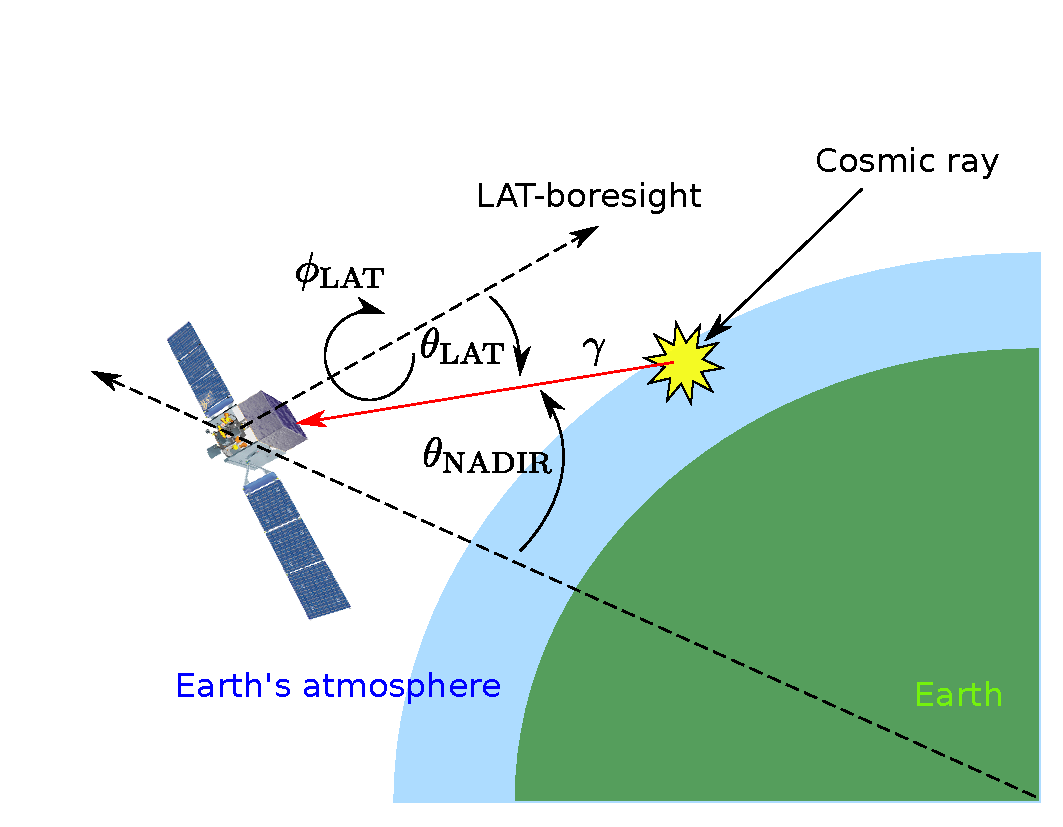
\includegraphics[width=0.7\textwidth]{img/gamma_production_schematic}
    \caption{Schematics of $\gamma$-ray production}
\end{figure}
Cosmic rays are high energic particles which are produced in space by various types
of acceleration mechanisms such as supernovae, active galactic nuclei, quasars, and
gamma-ray bursts. The main composition of CRs consist of 90\% protons, 8\% alpha
and other heavier atoms. The main reason that makes CRs spectrum follow power
law function in rigidity is the acceleration mechanism was dominated in
Lorenzian interaction which has a characeteristic spectral index.

\par CR spectrum has various spectral indices at different magnitude of energies, depending on the types of sources which can accelerate CRs to a certain energy range as shown in Figure \ref{fig:cr_famous_spectrum} \cite{Swordy2001}.
\begin{figure}[h!]
\centering
    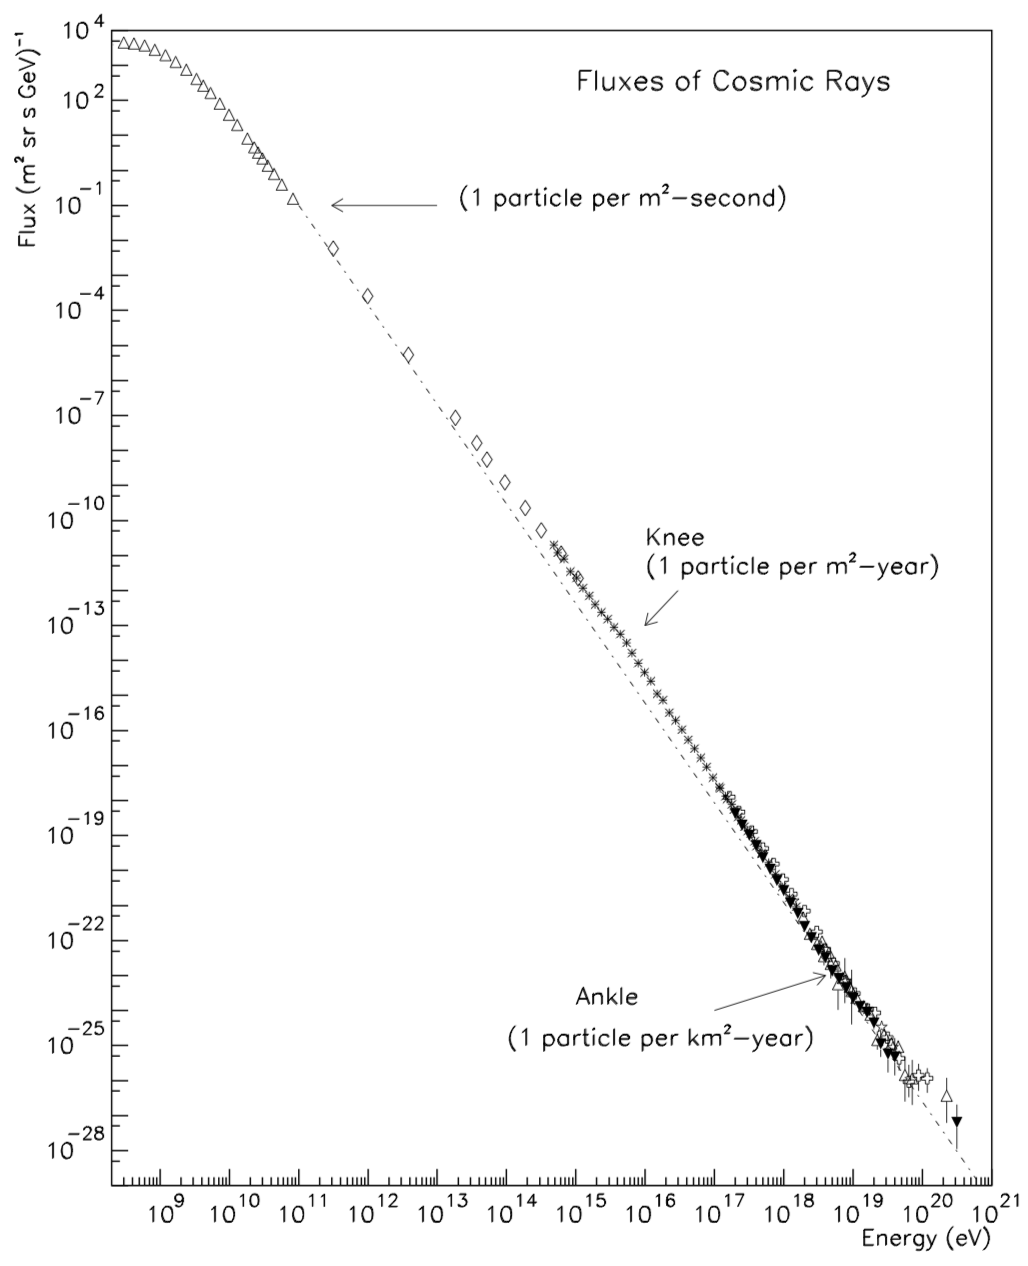
\includegraphics[width=0.6\textwidth]{img/Swordy}
    \caption{Main features of cosmic rays spectrum}
    \label{fig:cr_famous_spectrum}
\end{figure}

\par The motivation why we use $\gamma$-ray as a secondary product for investigate incident proton spectrum is that Earth limb's $\gamma$-ray relatively brigher than the sky due to collision from CRs in energy range 100 MeV and 1 TeV which consistent with our study \cite{Warit2009}.

\par Previous work has been performed using Pass 7 version data \cite{FermiPass7} and found an energy break point around 300 GeV with a significance of about 2$\sigma$ \cite{previouswork}. This result is consistent with direct measurements from \cite{AMS-02,PAMELA}.


\subsection{\textit{Fermi} Large Area Telescope}

Gamma-ray Large Area Space Telescope (GLAST) could be informally called \textit{Fermi}-LAT. The mission is to collect data of particles from multiple phenomena such as active galaxy nuclei (AGN), pulsars and other high energy sources.
It also attach the Gamma-ray Burst Monitor (GBM) to study gamma-ray bursts. Fermi was launched on 11 June 2008 at 16:05 UTC aboard a Delta II 7920-H rocket.


\subsubsection*{Instrument}
LAT consist with 16 layers of traker (TKR) modules, 16 calorimeter (CAL) and a parition ACD. 

\begin{figure}[h!]
  \centering
    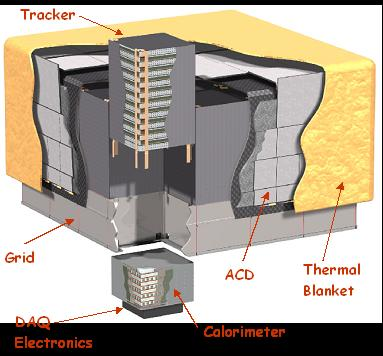
\includegraphics[width=0.5\textwidth]{img/LATStructure}
    \caption{Instrument structure : Image taken from https://fermi.gsfc.nasa.gov}
\end{figure}

\par TKR module has made from an array of silicon-strip tracking detectors (SSDs) and has 18 tracker on a horizontal planes. First 12 planes have 0.035 radiation lengths, next 4 layes contain 0.18 radiation lengths thick and the rest of it does not have any converter.
Tracking detector in each plane consist of two planar inner layer which running in x and y axis subsequently. The arrival $\gamma$-ray in LAT's field of view could produce electron-positron pair in TKR's plates.
The initial lepton pair could be determined from the recoed of conversion point in SSD planes with a power angular resolution when has a low energy.

\par Each CAL module contains 1536 CsI(Tl) crystal with an 96 crystal align in eight different orthogonal layers.
Dual PIN photodiodes also attach in each crystal which provide a great resolution in energy.

\par ACD tile contain wavelength shifting fiber by photomultiplier tubes (PMT) for redundancy. 
The tiles also are piled up in one direction.


\subsubsection*{Event reconstruction}
The methodlogy of detection is to track the lepton pair product from an incident photon that collide with a conversion foils and lepton produc be traced by second inner layer of TKR.
Consequently, the limit of precision depends on energy of photon that larger than mass energy of electron-positron as well as angle resolution of TKR that getting worser and worser at larger $\theta_\text{LAT}$.
Lastly, the lepton product could be measured the energy by a high precision crystal array in CAL. The event classification also divided into various level of confident event reconstruction with a different Instrument respondse function \cite{FermiDetail,Atwood:2013rka}.


\begin{figure}[h!]
  \centering
    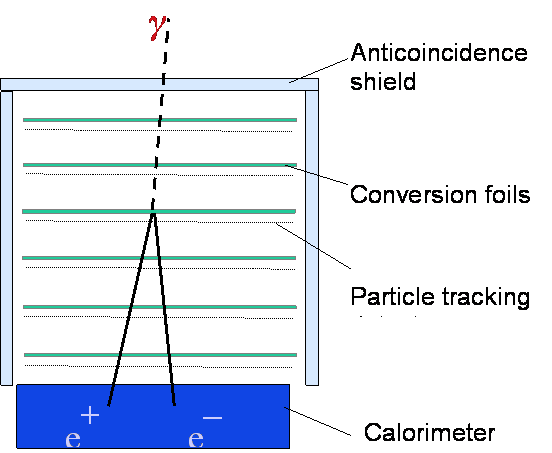
\includegraphics[width=0.5\textwidth]{img/LATMethodology}
    \caption{Schematic Structure of the LAT : Image taken from https://fermi.gsfc.nasa.gov}
  \end{figure}
